%%%%%%%%%%%%%%%%%%%%%%%%%%%%%%%%%%%%%%%%%
% baposter Landscape Poster
% LaTeX Template
% Version 1.0 (11/06/13)
%
% baposter Class Created by:
% Brian Amberg (baposter@brian-amberg.de)
%
% This template has been downloaded from:
% http://www.LaTeXTemplates.com
%
% License:
% CC BY-NC-SA 3.0 (http://creativecommons.org/licenses/by-nc-sa/3.0/)
%
%%%%%%%%%%%%%%%%%%%%%%%%%%%%%%%%%%%%%%%%%

%----------------------------------------------------------------------------------------
%	PACKAGES AND OTHER DOCUMENT CONFIGURATIONS
%----------------------------------------------------------------------------------------

\documentclass[landscape,a0paper,fontscale=0.3]{baposter} % Adjust the font scale/size here

\usepackage{graphicx} % Required for including images
\graphicspath{{/home/alli/projects/talks/figures/}} % Directory in which figures are stored

\usepackage{amsmath} % For typesetting math
\usepackage{amssymb} % Adds new symbols to be used in math mode
\usepackage{booktabs} % Top and bottom rules for tables
\usepackage{enumitem} % Used to reduce itemize/enumerate spacing
\usepackage{palatino} % Use the Palatino font
\usepackage[font=small,labelfont=bf]{caption} % Required for specifying captions to tables and figures

\usepackage{multicol} % Required for multiple columns
\setlength{\columnsep}{1.5em} % Slightly increase the space between columns
\setlength{\columnseprule}{0mm} % No horizontal rule between columns


\usepackage{tikz} % Required for flow chart
\usetikzlibrary{shapes,arrows} % Tikz libraries required for the flow chart in the template

\newcommand{\compresslist}{ % Define a command to reduce spacing within itemize/enumerate environments, this is used right after \begin{itemize} or \begin{enumerate}
\setlength{\itemsep}{1pt}
\setlength{\parskip}{0pt}
\setlength{\parsep}{0pt}
}

\definecolor{lightblue}{rgb}{0.145,0.6666,1} % Defines the color used for content box headers
\definecolor{darkpurple}{rgb}{0.28,0.24,0.55}


\begin{document}

\begin{poster}
{
%headerborder=closed, % Adds a border around the header of content boxes
colspacing=1em, % Column spacing
columns=3,
bgColorOne=white, % Background color for the gradient on the left side of the poster
bgColorTwo=white, % Background color for the gradient on the right side of the poster
borderColor=lightblue, % Border color
headerColorOne=darkgray, % Background color for the header in the content boxes (left side)
headerColorTwo=darkpurple, % Background color for the header in the content boxes (right side)
headerFontColor=white, % Text color for the header text in the content boxes
boxColorOne=white, % Background color of the content boxes
%textborder=roundedleft, % Format of the border around content boxes, can be: none, bars, coils, triangles, rectangle, rounded, roundedsmall, roundedright or faded
textborder=none, % Format of the border around content boxes, can be: none, bars, coils, triangles, rectangle, rounded, roundedsmall, roundedright or faded
eyecatcher=true, % Set to false for ignoring the left logo in the title and move the title left
headerheight=0.1\textheight, % Height of the header
%headershape=roundedright, % Specify the rounded corner in the content box headers, can be: rectangle, small-rounded, roundedright, roundedleft or rounded
headershape=rounded, % Specify the rounded corner in the content box headers, can be: rectangle, small-rounded, roundedright, roundedleft or rounded
headerfont=\Large\bf\textsc, % Large, bold and sans serif font in the headers of content boxes
%textfont={\setlength{\parindent}{1.5em}}, % Uncomment for paragraph indentation
linewidth=2pt % Width of the border lines around content boxes
}
%----------------------------------------------------------------------------------------
%	TITLE SECTION 
%----------------------------------------------------------------------------------------
%
{\includegraphics[height=6em]{illinois_logo.jpg}} % First university/lab logo on the left
{{Controllable~~Billiards:~~Characterizing~~the~~Paths~~of~~Simple~~Mobile~~Robots}\vspace{-0.0em}} % Poster title
{Alexandra Q. Nilles, Israel Becerra, Steven M. LaValle  \hspace{15pt}\\ Department of Computer Science, University of Illinois, Urbana-Champaign} % Author names and institution
{
\includegraphics[height=8em]{/home/alli/projects/talks/figures/nsf1.jpg}} % Second university/lab logo on the right

%----------------------------------------------------------------------------------------
%	INTRODUCTION
%----------------------------------------------------------------------------------------

\headerbox{Motivation}{name=intro,column=0,row=0,span=1}{

\begin{itemize}
\item What kinds of tasks can very simple robots perform?

\item What are the minimal resources (sensing, actuation, computation) needed to
complete tasks?

\item Can we make common robots such as vacuums, warehouse robots, etc more efficient
and robust?
\end{itemize}


\begin{center}
\includegraphics[width=1\linewidth]{robot_brain.jpg}
\end{center}


}

%----------------------------------------------------------------------------------------
%	Question
%----------------------------------------------------------------------------------------

\headerbox{Being Specific About Tasks}{name=question,below=intro,column=0,span=1}{

\begin{itemize}\compresslist
\item  
\item  
\item  
\item  
\end{itemize}

}

%----------------------------------------------------------------------------------------
%	MATERIALS AND METHODS 1
%----------------------------------------------------------------------------------------


\headerbox{Approach}{name=flow,column=0,span=1,below=question}{

Notice that many robots can travel forward in straight lines, identify when
they've reached a boundary (real or virtual), and turn in place!

Can we use billiards or similar models?

\begin{center}
\includegraphics[width=1\linewidth]{bounce_space_def.pdf}
\captionof{figure}{Outline of homology search and state mapping approach. Presence/absence patterns
are mapped onto the phylogenetic tree and ancestral gene combinations are
reconstructed in Count (Milk'{o}s Cs\H{u}r"{o}s, 2009) using Wagner parsimony
with a 1.1:1 gain:loss penalty. A penalty of 2 is typically used, but we assume 
that essential genes are less likely to be lost.}
\end{center}

}

%----------------------------------------------------------------------------------------
%	MATERIALS AND METHODS 2
%----------------------------------------------------------------------------------------


%\headerbox{Methods: Finding essential genes}{name=florida,column=1,span=1}{
%
%\begin{center}
%%\includegraphics[width=.85\linewidth]{florida_169.pdf}
%\includegraphics[width=1\linewidth]{./florida_serif.pdf}
%\captionof{figure}{A combination of heuristic (Solaimanpour, et al. 2015) and log-likelihood (Zomer, et al. 2012) methods revealed the essentialy 
%of genes based on their proportional representation in Tn-Seq data. 456 essential 
%gene candidates were underrepresented compared to the rest of the genome in both (green),
%and thus were classified as likely essential in rich medium.}
%
%\end{center}
%}
\headerbox{Results: Periodic Orbits in Convex Polygons}{name=circos,column=1,span=1}{

\begin{center}
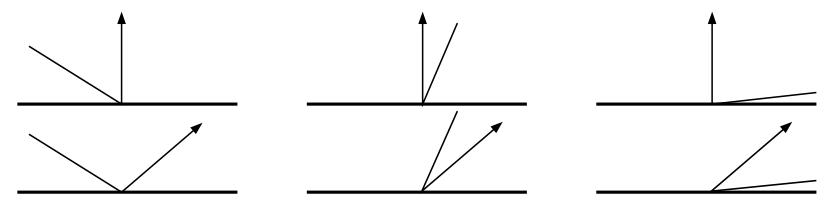
\includegraphics[width=1\linewidth]{bounce_examples.pdf}
\captionof{figure}{Circos plot of the genome (blue) with transposon insertions mapped onto it
(orange and green). Genes (red, middle) with significantly fewer insertions than
expected were called as essential (black).}


\end{center}
}



%----------------------------------------------------------------------------------------
%	RESULTS 1
%----------------------------------------------------------------------------------------

\headerbox{How to Approach Nonconvex Environments?}{name=heatmap,column=1,span=1}{ 

%\begin{multicols}{2}


\begin{center}
%\includegraphics[width=1\linewidth]{./heatmap_tag_colors_grid.pdf}
%\includegraphics[width=.85\linewidth]{./heatmap_tag_colors_grid_alt.pdf}
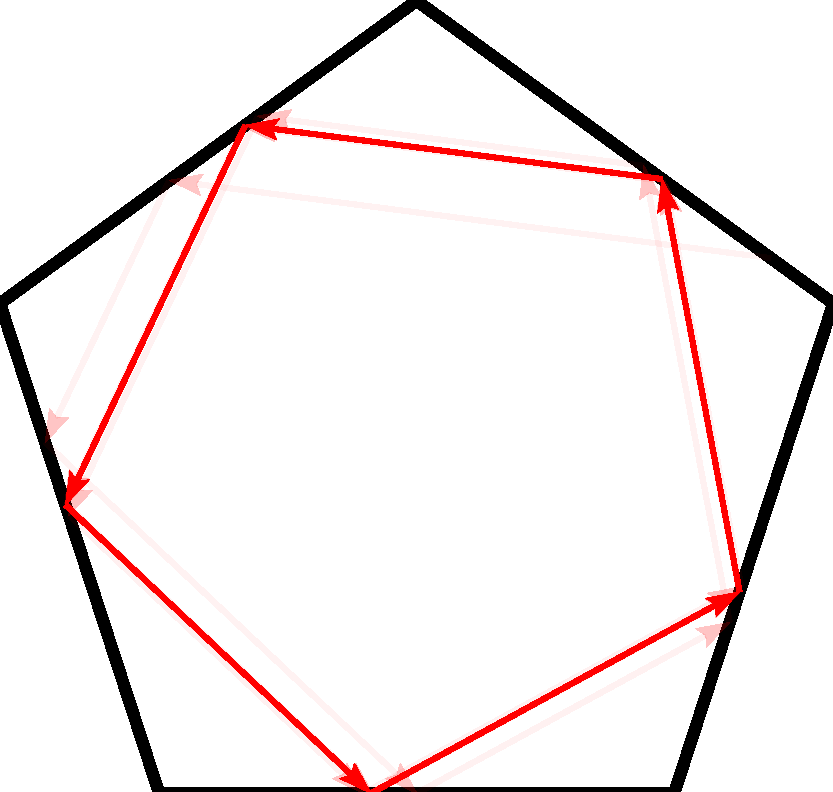
\includegraphics[width=1\linewidth]{pent_05rad.pdf}
\captionof{figure}{Presence (red) and absence (white) patters of essential genes (columns) across a diverse set of
genomes (rows), colors and species as in Figure 2) spanning major groups in each domain of life. }
\end{center}

}
%\end{multicols}


%----------------------------------------------------------------------------------------
%	RESULTS 2
%----------------------------------------------------------------------------------------
%\headerbox{Results: Reconstruciton}{name=results_2,column=2,span=1,below=circos}{ 
\headerbox{Chaotic Dynamics: Coverage Properties}{name=results_2,column=1,span=1}{ 


%%
%%\begin{multicols}{2}
\begin{center}
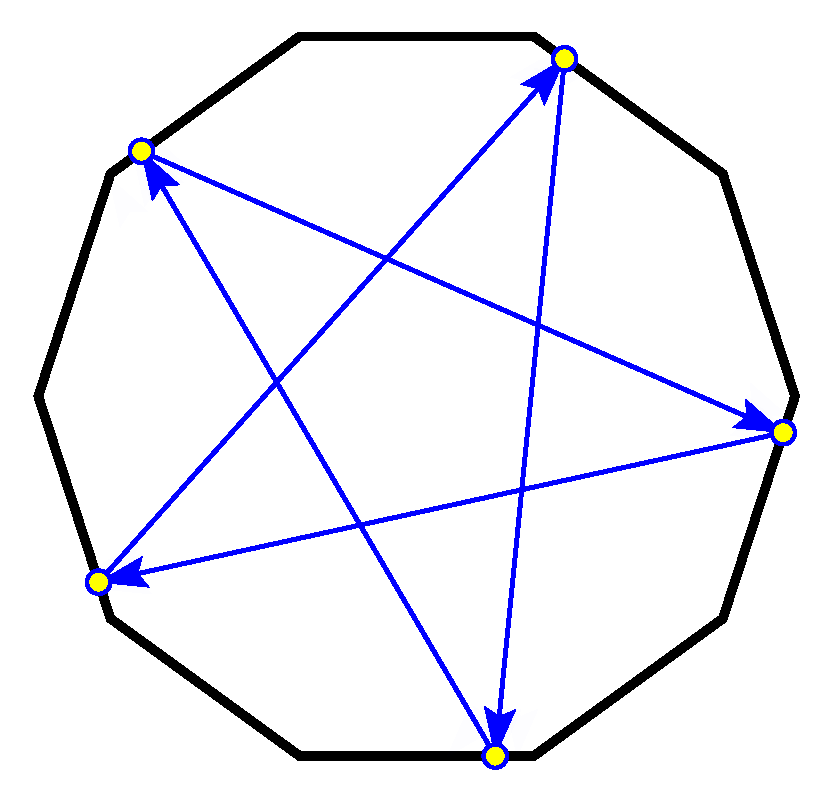
\includegraphics[width=0.95\linewidth]{../figs/nonagon_neg0pt8rad_skip3.pdf}
\captionof{figure}{Maximum parsimony tree made in PAUP\* (Swofford, et al 2017) from
presence/absence data (Figure 4). Distance represents gain/loss of essential
genes, and clustering represents shared gene sets. 1000 bootstraps were
performed and well-supported ancestral nodes were chosen for reconstruction (colored dots).
Bars represent the functional categories of \emph{S. islandicus} essential genes shared with that organism.}
\end{center}
}

%
%----------------------------------------------------------------------------------------
%	RESULTS 1
%----------------------------------------------------------------------------------------

%\headerbox{Results: Homology Search Across All Three Domains}{name=results_1,column=2,span=1}{
\headerbox{Results: Evolution of core systems}{name=results_1,column=2,span=1}{

\begin{center}
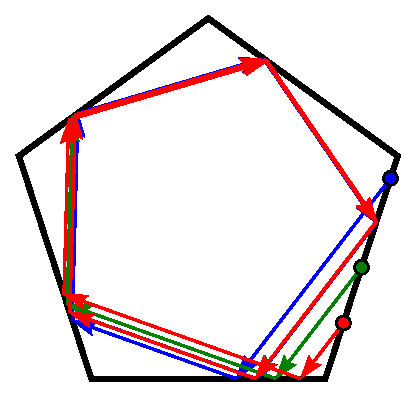
\includegraphics[width=1\linewidth]{../figs/multi_start.pdf}
\captionof{figure}{Genes predicted to be gained between certain common ancestors represent major
evolutionary transitions. 65\%  of the essential genome is predicted to have been
in place at or near the Last Universal Common Ancestor, and 76\% in the ancestor
with Eukaryotes. Archaeal inventions are primarily metabolic, involved in
defense mechanisms, or are uncharacterized.} 
\end{center}

}
%\begin{multicols}{2}
%
%
%\includegraphics[width=1\linewidth]{heatmap.pdf}
%\captionof{figure}{
%Putative homologs were found via all-against-all BLAST over 174 genomes.\
%Bidirectional best BLAST hits were aligned and used to make hidden Markov models\
%(HMMs), which scanned for more remote homologs and paralogs. Patterns of presence/absence, visible as large blocks, were then used to reconstruct ancestral states.\
%}
%
%%	\captionof{figure}{Putative homologs were found via all-against-all BLAST over 170 genomes. Bidirectional best BLAST hits were aligned and used to make hidden Markov models (HMMs). Here visualized are BBHs (blue) and HMM hits (green) across those genomes.}
%%\includegraphics[width=0.72\linewidth]{heatmap.pdf}
%\end{center}


%\begin{center}
%\includegraphics[width=.9\linewidth]{Timeline.pdf}
%\captionof{figure}{Number of M.16.4 genes in a specific arCOG category\textsuperscript{3} plotted along a hypothetical timeline based on phyletic patterns consistent with their presence in certain common ancestors. Future work will use these patterns to help trace the evolutionary history of key cell machinery, including isolating specific uncharacterized genes, determining their function, and inferring their role in the ancestral cell.}
%\end{center}

%\begin{center}
%	\includegraphics[width=.65\linewidth]{structure.pdf}
%	\captionof{figure}{Predicted structure of \textit{Sulfolobus} ZPR1 homolog. Sequence alignment (MAFFT) and structural threading (Phyre2) with mouse protein shows a high degree of conservation in key binding sites on the surface (red patches). In Eukaryotes, this protein plays an essential but uncharacterized role in constructing ribonucleoproteins and regulating cell cycle. }
%\end{center}


%\end{multicols}

%}
%----------------------------------------------------------------------------------------
%	RESULTS 3
%----------------------------------------------------------------------------------------
\headerbox{Results: Phylogeny}{name=results_3,column=2,span=1}{ 
%
\begin{center}
%\renewcommand\figurename{Table}
%\setcounter{figure}{0}
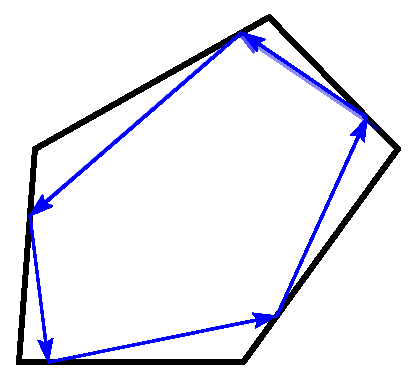
\includegraphics[width=1\linewidth]{../figs/shear.pdf}
\captionof{figure}{Universal genes were aligned with MAFFT, trimmed with TrimAl, and concatenated to produce a supermatrix, then this phylogenetic tree was constructed with RAxML. Consistent with 
patterns of gene gain and loss, this tree shows the separation of Archaea and Eukaryotes from Bacteria and the monophyly of the Archaea. Branch thickness corresponds with bootstrap value (1000 iterations).
Members of Asgardarchaeota, a candidate phyla of the Archaea hypothesized to be monophyletic with Eukaryotes, instead are with the Archaea in this analysis. }
%common ancestor of \emph{Igniogoccus hospitalis} and \emph{Sulfolobales} with two
%thermophilic bacterial species: \emph{Dictyoglomus thermophilum} H-6-12 and
%\emph{Thermodesulfovibrio yellowstonii} DSM 11347. 20 hypothetical proteins are also candidates for HGT with these bacteria (not shown).}
\end{center}
%
}
%\headerbox{Results: Reconstruciton}{name=results_2,column=2,span=1}{ 
%
%\begin{center}
%\includegraphics[width=1\linewidth]{./bars.pdf}
%\captionof{figure}{Functional breakdown of genes placed at certain common ancestors shows a largely mature cell by the time of the last ancestor with Eukaryotes.}
%\end{center}
%
%}
%----------------------------------------------------------------------------------------
%	CONCLUSIONS
%----------------------------------------------------------------------------------------

\headerbox{Conclusions}{name=conclusions,column=2,span=1}{ 
\begin{itemize}\compresslist
\item Most of the ancestral genome was present in Last Eukaryotic and Archaeal common ancestor
\item Archaea are still monophyletic in these analyses, suggesting a separate origin or massive gene loss in Eukaryota.
\item \emph{Sulfolobales} have undergone much uncharacterized gene innovation since split from Crenarchaeota. 
\end{itemize}
}



%----------------------------------------------------------------------------------------
%	FUTURE DIRECTIONS
%----------------------------------------------------------------------------------------

%\headerbox{Future Directions}{name=future,column=3,span=1,below=conclusions}{ 
%\begin{itemize}\compresslist
%\item Add other archaeal phyla to the analysis.
%\item Construct gene trees and compare species trees generated from different cellular systems.
%\item Use gene trees to test predicted HGT.
%\item Experimentally study uncharactarized essential genes unique to \emph{Sulfolobus} or shared between Archaea and Eukaryotes.
%\end{itemize}
%}



%----------------------------------------------------------------------------------------
%----------------------------------------------------------------------------------------
%	ACKNOWLEDGMENTS
%----------------------------------------------------------------------------------------

\headerbox{Acknowledgments}{name=acknowledgments,column=2,span=1,above=bottom}{
\small{
\textbf{Graduate Committee:} Rachel~Whitaker, Peter~Orlean, Gary~Olsen, William~Metcalf, and Isaac~Cann \\
\textbf{Undergraduates}: Rebecca~Wipfler, Angelo~Blancaflor, and Carlos~Vega \\
\textbf{Annotation} help from Dr.~Kira~Makarova of the NCBI\\
\textbf{Funding} from the NASA Astrobiology Institute and the Carl R. Woese Institute for Genomic Biology.
}


}
%----------------------------------------------------------------------------------------
%	REFERENCES
%----------------------------------------------------------------------------------------

%\headerbox{References}{name=references,column=1,above=bottom}{
%
%\tiny{
%
%
%1. Woese, C., et al. PNAS, 4576–4579 (1990).\\
%2. Zomer, A., et al. PLoS ONE 7, e43012 (2012).\\
%3. Solaimanpour, S., et al. PLOS ONE 10, e0126070 (2015).\\
%4. Makarova, K., , et al. Life 5, 818–840 (2015).
%
%
%}}
%
%----------------------------------------------------------------------------------------
%	FUTURE RESEARCH
%----------------------------------------------------------------------------------------
%
%\headerbox{Future Research}{name=futureresearch,column=1,span=2,aligned=references,above=bottom}{ % This block is as tall as the references block
%
%\begin{multicols}{2}
%Integer sed lectus vel mauris euismod suscipit. Praesent a est a est ultricies pellentesque. Donec tincidunt, nunc in feugiat varius, lectus lectus auctor lorem, egestas molestie risus erat ut nibh.
%
%Maecenas viverra ligula a risus blandit vel tincidunt est adipiscing. Suspendisse mollis iaculis sem, in \emph{imperdiet} orci porta vitae. Quisque id dui sed ante sollicitudin sagittis.
%\end{multicols}
%}
%




\end{poster}

\end{document}
